

\chapter{数值结果验证}

\section{基准算例概述}

为了验证\ProgramName 程序的临界计算及时空动力学计算功能,
本章使用常用的三个不含热工反馈的时空动力学基准题对程序的结果进行验证。
临界计算的对比程序选用广泛使用的细网有限差分多群扩散程序——Citation。

\subsection{静态IAEA PWR三维基准问题}
\label{sec:result.test.iaea}

IAEA 三维压水堆基准题是三维两群扩散基准题\cite{center1977benchmark},
由177个燃料组件构成,堆芯取$1/4$,
大小为170cm $\times$ 170cm $\times$ 380cm,
堆芯的几何结构见\floatref{fig:result.test.iaea},
堆芯中心为对称边界条件,外侧边界入流为0,外侧也可取等效边界条件
\begin{align}
  \frac{\partial \phi_g}{\partial n}=-\frac{0.4692}{D_g}\phi_g
\end{align}

各材料界面见\floatref{tab:result.test.iaea.mat},
裂变谱取$\chi_1=1$,$\chi_2=0$。

\begin{table}
\centering
\caption{\label{tab:result.test.iaea.mat}静态IAEA PWR 三维基准题材料截面}
\begin{tabular}{cccccc}
\toprule
材料 & 能群$g$ & $D_g/\mathrm{cm}$ & $\Sigma_{a,g}/\mathrm{cm}^{-1}$
    & $\nu\Sigma_{f,g}/n,\mathrm{cm}^{-1}$
    & $\Sigma_{s,1\rightarrow2}/\mathrm{cm}^{-1}$\\
\midrule
\multirow{2}{*}{M1} 
  & 1 & 1.5 & 0.01 & 0 & \multirow{2}{*}{0.02} \\
  & 2 & 0.4 & 0.08 & 0.135 &\\
\multirow{2}{*}{M2} 
  & 1 & 1.5 & 0.01 & 0 & \multirow{2}{*}{0.02} \\
  & 2 & 0.4 & 0.085 & 0.135 &\\
\multirow{2}{*}{M3} 
  & 1 & 1.5 & 0.01 & 0 & \multirow{2}{*}{0.02} \\
  & 2 & 0.4 & 0.13 & 0.135 &\\
\multirow{2}{*}{M4} 
  & 1 & 2.0 & 0 & 0 & \multirow{2}{*}{0.04} \\
  & 2 & 0.3 & 0.01 & 0 &\\
\multirow{2}{*}{M5} 
  & 1 & 2.0 & 0 & 0 & \multirow{2}{*}{0.04} \\
  & 2 & 0.3 & 0.055 & 0 &\\
\bottomrule
\end{tabular}
\end{table}

\begin{figure}
\centering
\begin{subfigure}{\textwidth}
\centering
\begin{tikzpicture}[scale=0.7, transform shape]
\def\lenscale{0.06}

\def\x#1{#1*\lenscale}
\def\zz#1{#1*\lenscale-8}
\def\z#1{#1*\lenscale}

\draw [very thick] (0,0) -- (\x{170},0) 
            -- (\x{170}, \zz{380}) -- (0, \zz{380});
\draw [loosely dashdotted] (0,0) -- (0, \zz{380});
\draw (0,\z{20}) -- (\x{150},\z{20}) -- (\x{150},\zz{360}) -- (0,\zz{360});
\draw (\x{10},\z{20}) -- (\x{10},\zz{380});
\draw [dashed] (\x{30},\zz{380}) -- (\x{30},\zz{280}) -- (\x{50},\zz{280}) -- (\x{50},\zz{380});
\draw (\x{70},\z{20}) -- (\x{70},\zz{380});
\draw (\x{90}, \z{20}) -- (\x{90},\zz{380});
\draw (\x{130},\z{20}) -- (\x{130},\zz{360});
\node at (\x{10},\z{80}) {\huge $\approx$};
\node at (\x{70},\z{80}) {\huge $\approx$};
\node at (\x{90},\z{80}) {\huge $\approx$};
\node at (\x{130},\z{80}) {\huge $\approx$};
\node at (\x{150},\z{80}) {\huge $\approx$};
\node at (\x{170},\z{80}) {\huge $\approx$};

\node [left] at (0,0) {\Large 0};
\node [left] at (0,\z{20}) {\Large 20};
\node [left] at (0,\zz{280}) {\Large 280};
\node [left] at (0,\zz{360}) {\Large 360};
\node [left] at (0,\zz{380}) {\Large 380};

\foreach \xp in {0, 10,30,50,70,90,130,150,170}
{
\node [above] at (\x{\xp},\zz{380}) {\Large \xp};
}

\node at (\x{160}, \zz{260}) {\Large M4};
\node at (\x{140}, \zz{260}) {\Large M1};
\node at (\x{110}, \zz{260}) {\Large M2};
\node at (\x{80}, \zz{260}) {\Large M3};
\node at (\x{40}, \zz{260}) {\Large M2};

\draw [-latex new, arrow head=3mm] (-1,\zz{260}) -- (\x{5}, \zz{260});
\node [left] at (-1, \zz{260}) {\Large M3};

%\draw [-latex new, arrow head=3mm] (-1,\zz{320}) -- (\x{40}, \zz{320});
%\node [left] at (-1, \zz{320}) {\Large Mp3};
\node at (\x{40}, \zz{320}) {\Large M3};

\node at (\x{80}, \zz{370}) {\Large M5};
\node at (\x{60}, \zz{370}) {\Large M4};
\node at (\x{40}, \zz{370}) {\Large M5};
\node at (\x{20}, \zz{370}) {\Large M4};

\draw [-latex new, arrow head=3mm] (-1,\zz{370}) -- (\x{5}, \zz{370});
\node [left] at (-1, \zz{370}) {\Large M5};

\node [above] at (-0.5,\zz{380}+0.5) {\Large cm};
\node [above] at (\x{170}+1,\zz{380}) {\Large cm};
\end{tikzpicture}
\caption{纵截面图}
\end{subfigure}
\begin{subfigure}{\textwidth}
\centering
\begin{tikzpicture}[scale=0.7, transform shape]
\def\lenscale{0.06}
\def\x#1{#1*\lenscale}

\draw [loosely dashdotted] (\x{170},0) -- (0,0) -- (0,\x{170});
%\draw [loosely dashdotted] (0,0) -- (\x{170},\x{170});

\draw (\x{10},0) -- (\x{10},\x{10}) -- (0,\x{10});

\draw (\x{70},0) -- (\x{70},\x{10}) -- (\x{90},\x{10}) -- (\x{90},0);
\draw (0,\x{70}) -- (\x{10},\x{70}) -- (\x{10},\x{90}) -- (0,\x{90});
\node [left] at (-1,\x{80}) {\Large M3};
\draw [-latex new, arrow head=3mm] (-1,\x{80}) -- (\x{5}, \x{80});
\node at (\x{80},\x{5}) {\Large M3};

\draw (\x{30},\x{30}) rectangle (\x{50},\x{50});
\node at (\x{40},\x{40}) {\Large M3};

\draw (0,\x{130}) -- (\x{30},\x{130}) -- (\x{30},\x{110})
           -- (\x{70},\x{110}) -- (\x{70},\x{70})
           -- (\x{110},\x{70}) -- (\x{110},\x{30})-- (\x{130},\x{30})
           -- (\x{130},0);
\node at (\x{40},\x{80}) {\Large M2};

\draw (\x{70},\x{70}) rectangle (\x{90},\x{90});
\node at (\x{80},\x{80}) {\Large M3};

\draw (0,\x{150}) -- (\x{50},\x{150}) -- (\x{50},\x{130})
           -- (\x{90},\x{130}) -- (\x{90},\x{110})
           -- (\x{110},\x{110})
           -- (\x{110},\x{90}) -- (\x{130},\x{90})-- (\x{130},\x{50})
           -- (\x{150},\x{50}) -- (\x{150},0);
\node at (\x{50},\x{120}) {\Large M1};

\draw [very thick] (0,\x{170}) -- (\x{70},\x{170}) -- (\x{70},\x{150})
           -- (\x{110},\x{150}) -- (\x{110},\x{130})
           -- (\x{130},\x{130})
           -- (\x{130},\x{110}) -- (\x{150},\x{110})-- (\x{150},\x{70})
           -- (\x{170},\x{70}) -- (\x{170},0);
\node at (\x{70},\x{140}) {\Large M4};

\foreach \xp in {0, 10,30,50,70,90,130,150,170}
{
\node [below] at (\x{\xp},0) {\Large \xp};
\node [left] at (0,\x{\xp}) {\Large \xp};
}

\node [below] at (\x{170}+1,0) {\Large cm};
\node [left] at (0, \x{170}+0.5) {\Large cm};

\draw [-latex new, arrow head=3mm](-1,\x{5}) -- (\x{5},\x{5});
\node [left] at (-1,\x{5}) {\Large M3};

\end{tikzpicture}
\caption{横截面图}
\end{subfigure}
\caption{\label{fig:result.test.iaea}静态IAEA PWR 三维基准题堆芯几何}
\end{figure}

\FloatBarrier
\subsection{动态TWIGL二维基准问题}
\label{sec:result.test.twigl}
TWIGL是二维两群扩散时空动力学基准题,
在1969年由Hageman和Yasinsky
于文献\onlinecite{hageman1969comparison}中提出\cite{gehin1992quasi},
堆芯取$1/4$,大小为80cm $\times$ 80cm,
堆芯的几何结构见\floatref{fig:result.test.twigl},
堆芯中心为对称边界条件,外侧边界入流为0。

各材料截面见\floatref{tab:result.test.twigl.mat},
裂变谱和缓发中子谱取$\chi_1=1$,$\chi_2=0$。
群速度为
\begin{align}
  \left\{
  \begin{aligned}
  v_1&=1.0\times10^7\mathrm{cm/s}\\
  v_2&=2.0\times10^5\mathrm{cm/s}
  \end{aligned}
  \right.
\end{align}
缓发中子为单组缓发中子
\begin{align}
  \left\{
  \begin{aligned}
  \beta&=0.0075\\
  \lambda&=0.08\mathrm{s}^{-1}
  \end{aligned}
  \right.
\end{align}
反应性引入方式
\begin{enumerate}
\item 阶跃引入:
\begin{align}
\Delta\Sigma_{a,2}&=-0.0035\mathrm{cm}^{-1} \quad t=0
\end{align}

\item 线性引入:
\begin{align}
\Sigma_{a,2}(t)&=\begin{cases}
    (1-0.11667t)\Sigma_{a,2}(0) & t\le 0.2\\
    0.97666\Sigma_{a,2}(0) & t > 0.2
  \end{cases}
\end{align}


\end{enumerate}

\begin{table}
\centering
\caption{\label{tab:result.test.twigl.mat}动态TWIGL二维基准题材料截面}
\begin{tabular}{cccccc}
\toprule
材料 & 能群$g$ & $D_g/\mathrm{cm}$ & $\Sigma_{a,g}/\mathrm{cm}^{-1}$
    & $\nu\Sigma_{f,g}/n,\mathrm{cm}^{-1}$
    & $\Sigma_{s,1\rightarrow2}/\mathrm{cm}^{-1}$\\
\midrule
\multirow{2}{*}{M1} 
  & 1 & 1.4 & 0.01 & 0.007 & \multirow{2}{*}{0.01} \\
  & 2 & 0.4 & 0.15 & 0.2 &\\
\multirow{2}{*}{M2} 
  & 1 & 1.4 & 0.01 & 0.007 & \multirow{2}{*}{0.01} \\
  & 2 & 0.4 & 0.15 & 0.2 &\\
\multirow{2}{*}{M3} 
  & 1 & 1.3 & 0.008 & 0.003 & \multirow{2}{*}{0.01} \\
  & 2 & 0.5 & 0.05 & 0.06 &\\
\bottomrule
\end{tabular}
\end{table}

\begin{figure}
\centering
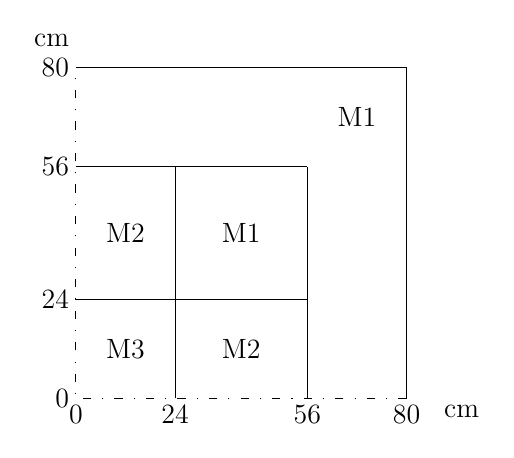
\begin{tikzpicture}[scale=0.7, transform shape]
\def\lenscale{0.075}
\def\x#1{#1*\lenscale}

\draw [loosely dashdotted] (\x{80},0) -- (0,0) -- (0,\x{80});

\draw (\x{24},0) -- (\x{24},\x{56});
\draw (0,\x{24}) -- (\x{56},\x{24});
\draw (\x{56},0) -- (\x{56},\x{56});
\draw (0,\x{56}) -- (\x{56},\x{56});
\draw (\x{80},0) -- (\x{80},\x{80});
\draw (0,\x{80}) -- (\x{80},\x{80});

\node at (\x{12},\x{12}) {\Large M3};
\node at (\x{40},\x{12}) {\Large M2};
\node at (\x{12},\x{40}) {\Large M2};
\node at (\x{40},\x{40}) {\Large M1};
\node at (\x{68},\x{68}) {\Large M1};

\foreach \xp in {0, 24, 56,80}
{
\node [below] at (\x{\xp},0) {\Large \xp};
\node [left] at (0,\x{\xp}) {\Large \xp};
}

\node [below] at (\x{80}+1,0) {\Large cm};
\node [left] at (0, \x{80}+0.5) {\Large cm};

\end{tikzpicture}
\caption{\label{fig:result.test.twigl}动态TWIGL二维基准题堆芯几何}
\end{figure}

\FloatBarrier
\subsection{动态LMW三维基准问题}

LMW(Langenbuch-Maurer-Werner)基准题\cite{langenbuch1977coarse,gehin1992quasi}是
三维两群扩散中子时空动力学基准题,
大小为$1/4$堆芯,几何尺寸110cm $\times$ 110cm $\times$ 200cm,
见\floatref{fig:result.test.lmw}。

\begin{figure}
\centering
\begin{subfigure}{.45\textwidth}
\hspace{-1.5cm}
\begin{tikzpicture}[scale=0.7, transform shape]
\def\lenscale{0.075}
\def\x#1{#1*\lenscale}

\draw [loosely dashdotted] (\x{110},0) -- (0,0) -- (0,\x{110});

\draw (\x{10},\x{0}) -- (\x{10},\x{10}) -- (\x{0},\x{10});
\draw (\x{50},\x{0}) -- (\x{50},\x{10}) -- (\x{70},\x{10}) -- (\x{70},\x{0});
\draw (\x{0},\x{50}) -- (\x{10},\x{50}) -- (\x{10},\x{70}) -- (\x{0},\x{70});
\node at (\x{30},\x{10}) {\Large M1};
\node at (\x{60},\x{5}) {\Large M2};
\node at (\x{5},\x{60}) {\Large M2};
\node at (\x{5},\x{5}) {\Large M2};

\draw (\x{30},\x{30}) rectangle (\x{50},\x{50});
\node at (\x{40},\x{40}) {\Large M2};

\draw (\x{70},\x{0}) -- (\x{70},\x{50}) -- (\x{50},\x{50})
      -- (\x{50},\x{70}) -- (\x{0},\x{70});
\node at (\x{60},\x{60}) {\Large M3};

\draw (\x{90},\x{0}) -- (\x{90},\x{70}) -- (\x{70},\x{70})
      -- (\x{70},\x{90}) -- (\x{0},\x{90});
\node at (\x{80},\x{80}) {\Large M4};

\draw (\x{110},\x{0}) -- (\x{110},\x{90}) -- (\x{90},\x{90})
      -- (\x{90},\x{110}) -- (\x{0},\x{110});

\foreach \xp in {0, 10,30,50,70,90,110}
{
\node [below] at (\x{\xp},0) {\Large \xp};
\node [left] at (0,\x{\xp}) {\Large \xp};
}

\node [below] at (\x{110}+1,0) {\Large cm};
\node [left] at (0, \x{110}+0.5) {\Large cm};

\draw [-latex new, arrow head=3mm] (-1.25,\x{50}) -- (\x{0},\x{60});
\draw [-latex new, arrow head=3mm] (-1.25,\x{50}) -- (\x{60},\x{10});
\node [left] at (-1.25,\x{50}) {\Large 第一组};

\draw [-latex new, arrow head=3mm] (-1.25,\x{20}) -- (\x{5},\x{10});
\draw [-latex new, arrow head=3mm] (-1.25,\x{20}) -- (\x{30},\x{40});
\node [left] at (-1.25,\x{20}) {\Large 第二组};

\end{tikzpicture}
\caption{横截面图}
\end{subfigure}
\\[1cm]
\begin{subfigure}{.45\textwidth}
\begin{tikzpicture}[scale=0.7, transform shape]
\def\lenscale{0.06}

\def\x#1{#1*\lenscale}
\def\zz#1{#1*\lenscale}
\def\z#1{#1*\lenscale}

\draw [very thick] (0,0) -- (\x{110},0) 
            -- (\x{110}, \zz{200}) -- (0, \zz{200});
\draw [loosely dashdotted] (0,0) -- (0, \zz{200});

\draw (0,\z{20}) -- (\x{90},\z{20}) -- (\x{90},\x{180}) -- (0,\zz{180});
\draw (\x{70},\x{20}) -- (\x{70},\x{180});

\node [left] at (0,0) {\Large 0};
\node [left] at (0,\z{20}) {\Large 20};
\node [left] at (0,\z{60}) {\Large 60};
\node [left] at (0,\z{100}) {\Large 100};
\node [left] at (0,\zz{180}) {\Large 180};
\node [left] at (0,\zz{200}) {\Large 200};

\node at (\x{30},\x{40}) {\Large M1};
\node at (\x{80},\x{100}) {\Large M3};
\node at (\x{100},\x{100}) {\Large M4};
\node at (\x{20},\x{190}) {\Large M4};
\node at (\x{40},\x{190}) {\Large M2};
\node at (\x{60},\x{190}) {\Large M2};
\draw [-latex new, arrow head=3mm] (-1,\x{190}) -- (\x{5},\x{190});
\node [left] at (-1,\x{190}) {\Large M2};

\draw [dashed] (\x{0},\x{100}) -- (\x{10},\x{100}) -- (\x{10},\x{200});
\draw (\x{10},\x{180}) -- (\x{10},\x{200});
\draw (\x{50},\x{200}) -- (\x{50},\x{100}) -- (\x{70},\x{100}) -- (\x{70},\x{200});
\draw [dashed] (\x{30},\x{180}) -- (\x{30},\x{200});

\node at (\x{60},\x{140}) {\Large M2};
\draw [-latex new, arrow head=3mm] (-1,\x{140}) -- (\x{5},\x{140});
\node [left] at (-1,\x{140}) {\Large M2};

\draw [-latex new, arrow head=3mm] (-1,\x{70}) -- (\x{5},\x{100});
\draw [-latex new, arrow head=3mm] (-1,\x{70}) -- (\x{60},\x{100});
\node [left] at (-1,\x{70}) {\Large 第一组};
\draw [-latex new, arrow head=3mm] (-1,\x{160}) -- (\x{5},\x{180});
\draw [-latex new, arrow head=3mm] (-1,\x{160}) -- (\x{40},\x{180});
\node [left] at (-1,\x{160}) {\Large 第二组};

\foreach \xp in {0,10,30,50,70,90,110}
{
\node [above] at (\x{\xp},\zz{200}) {\Large \xp};
}

\node at (-0.75,\zz{200}+0.75) {\Large cm};
\end{tikzpicture}
\caption{纵截面图(初始时控制棒位置)}
\end{subfigure}
\begin{subfigure}{.45\textwidth}
\begin{tikzpicture}[scale=0.7, transform shape]
\def\lenscale{0.06}

\def\x#1{#1*\lenscale}
\def\zz#1{#1*\lenscale}
\def\z#1{#1*\lenscale}

\draw [very thick] (0,0) -- (\x{110},0) 
            -- (\x{110}, \zz{200}) -- (0, \zz{200});
\draw [loosely dashdotted] (0,0) -- (0, \zz{200});

\draw (0,\z{20}) -- (\x{90},\z{20}) -- (\x{90},\x{180}) -- (0,\zz{180});
\draw (\x{70},\x{20}) -- (\x{70},\x{180});

\node [left] at (0,0) {\Large 0};
\node [left] at (0,\z{20}) {\Large 20};
\node [left] at (0,\z{60}) {\Large 60};
\node [left] at (0,\z{100}) {\Large 100};
\node [left] at (0,\zz{180}) {\Large 180};
\node [left] at (0,\zz{200}) {\Large 200};

\node at (\x{30},\x{40}) {\Large M1};
\node at (\x{80},\x{100}) {\Large M3};
\node at (\x{100},\x{100}) {\Large M4};
\node at (\x{20},\x{190}) {\Large M4};
\node at (\x{40},\x{190}) {\Large M2};
\node at (\x{60},\x{190}) {\Large M2};
\draw [-latex new, arrow head=3mm] (-1,\x{190}) -- (\x{5},\x{190});
\node [left] at (-1,\x{190}) {\Large M2};

\draw (\x{0},\x{60}) -- (\x{10},\x{60}) -- (\x{10},\x{200});
\draw [dashed] (\x{30},\x{200}) -- (\x{30},\x{60}) -- (\x{50},\x{60}) -- (\x{50},\x{200});
\draw (\x{50},\x{180}) -- (\x{50},\x{200});
\draw (\x{70},\x{180}) -- (\x{70},\x{200});

\draw [-latex new, arrow head=3mm] (-1,\x{30}) -- (\x{5},\x{60});
\draw [-latex new, arrow head=3mm] (-1,\x{30}) -- (\x{40},\x{60});
\node [left] at (-1,\x{30}) {\Large 第二组};
\draw [-latex new, arrow head=3mm] (-1,\x{160}) -- (\x{5},\x{180});
\draw [-latex new, arrow head=3mm] (-1,\x{160}) -- (\x{60},\x{180});
\node [left] at (-1,\x{160}) {\Large 第一组};

\node at (\x{40},\x{120}) {\Large M2};
\draw [-latex new, arrow head=3mm] (-1,\x{120}) -- (\x{5},\x{120});
\node [left] at (-1,\x{120}) {\Large M2};

\foreach \xp in {0,10,30,50,70,90,110}
{
\node [above] at (\x{\xp},\zz{200}) {\Large \xp};
}

\node at (-0.75,\zz{200}+0.75) {\Large cm};
\end{tikzpicture}
\caption{纵截面图(最终控制棒位置)}
\end{subfigure}
\caption{\label{fig:result.test.lmw}动态LMW三维基准题堆芯几何}
\end{figure}

\begin{table}
\centering
\caption{\label{tab:result.test.lmw.mat}动态LMW三维基准题材料截面}
\begin{tabular}{cccccc}
\toprule
材料 & 能群$g$ & $D_g/\mathrm{cm}$ & $\Sigma_{a,g}/\mathrm{cm}^{-1}$
    & $\nu\Sigma_{f,g}/n,\mathrm{cm}^{-1}$
    & $\Sigma_{s,1\rightarrow2}/\mathrm{cm}^{-1}$\\
\midrule
\multirow{2}{*}{M1} 
  & 1 & 1.423913 & 0.01040206 & 0.006477691 & \multirow{2}{*}{0.0175555} \\
  & 2 & 0.356306 & 0.08766217 & 0.1127328 &\\
\multirow{2}{*}{M2} 
  & 1 & 1.423913 & 0.01095206 & 0.006477691 & \multirow{2}{*}{0.0175555} \\
  & 2 & 0.356306 & 0.09146217 & 0.1127328 &\\
\multirow{2}{*}{M3} 
  & 1 & 1.425611 & 0.01099263 & 0.007503284 & \multirow{2}{*}{0.01717768} \\
  & 2 & 0.350574 & 0.09925634 & 0.1378004 &\\
\multirow{2}{*}{M4} 
  & 1 & 1.634227 & 0.002660573 & 0 & \multirow{2}{*}{0.02759693} \\
  & 2 & 0.264002 & 0.04936351 & 0 &\\
\bottomrule
\end{tabular}
\end{table}


算例包含两组控制棒,开始时第一组控制棒以3cm/s的速度拔出,
26.67s时停止。第二组控制棒从7.5s开始以同样的速度插入,47.5s时停止,
控制棒位置随时间变化见\floatref{fig:result.test.lmw.rob}。
\begin{figure}
\centering
\includegraphics[scale=0.9]{result-test-lmw-rob}
\caption{\label{fig:result.test.lmw.rob}LMW算例控制棒位置随时间变化图}
\end{figure}

裂变谱和缓发中子谱取$\chi_1=1$,$\chi_2=0$。
群速度为
\begin{align}
  \left\{
  \begin{aligned}
  v_1&=1.25\times10^7\mathrm{cm/s}\\
  v_2&=2.5\times10^5\mathrm{cm/s}
  \end{aligned}
  \right.
\end{align}
缓发中子有6组,见\floatref{tab:result.test.lmw.mat.c}。

\begin{table}
\centering
\caption{\label{tab:result.test.lmw.mat.c}动态LMW三维基准题缓发中子数据}
\begin{tabular}{ccc}
\toprule
缓发中子组 & 缓发中子份额$\beta_i$ & 衰变常数$\lambda_i/\mathrm{s}^{-1}$\\
\midrule
1 & 0.000247 & 0.0127\\
2 & 0.0013845 & 0.0317\\
3 & 0.001222 & 0.1150\\
4 & 0.0026455 & 0.3110\\
5 & 0.000832 & 1.400\\
6 & 0.000169 & 3.870\\
\bottomrule
\end{tabular}
\end{table}


\section{数值结果验证}

在比较\ProgramName 的计算结果和参考结果之前,
先介绍本文使用的通量结果偏差的计算方式。

对于临界问题,程序计算得到的通量分布结果的绝对值无意义,
有意义的是各网格上通量的相对大小关系,
所以一般都需要对结果进行归一化,
再比较归一化后的通量结果。
那么选择的归一化方法就会影响到计算结果的对比,
常见的归一化方式是总功率归一化和最大通量归一化,
但这两种方法都有各自的问题:
由于堆芯中通量分布在不同的网格上可相差数个量级,
如果按照堆芯总功率进行归一化,那么堆芯中部功率较高的部分对归一化系数影响很大,
高通量区域的误差会通过归一化系数转移到到低通量区域上;
同理使用最大通量归一化时,通量最高处的误差会影响到其他所有点的误差结果。
在常见的组件级通量统计中,这种问题并不明显,
但在细网结果的相对误差比较中,这种影响就被放大了。

为了减小高通量网格对归一化系数的影响,本文使用所有网格上的相对幅值的均值作为
归一化系数,即待验证的通量分布$\phi$和参考通量分布$\psi$间的相对归一化系数取为
\begin{align}
  \eta = \frac{\ \displaystyle\sum_{\bm{k},g}\frac{\phi_{\bm{k},g}}{\psi_{\bm{k},g}}\ }
              {\displaystyle\sum_{\bm{k},g}1}
\end{align}
其中$\bm{k}$为空间网格编号,
则归一化后的各网格的最大相对误差为
\begin{align}
  e_\mathrm{max} = \max_{\bm{k},g}
      \left|
        \frac{\phi_{\bm{k},g}}{\eta\cdot\psi_{\bm{k},g}} - 1
      \right|
\end{align}
本文以后提到的最大相对误差均是指上式所定义的最大相对误差,
而且为了更好地反映有实际意义的堆芯内的通量的相对误差,
一般把堆芯活性区以外的水反射层处通量极低的网格滤掉。

本文中如无特殊声明,计算环境均为
\begin{itemize}
\item CPU: 2$\times$ Intel Xeon CPU X5670 2.93GHz (双路服务器)
\item 内存:24GB
\item GPU:NVIDIA GeForce GTX TITAN,6GB显存
\item 操作系统:Windows 7 SP1 64位
\end{itemize}

\subsection{静态IAEA PWR三维基准题}

使用Citation的计算结果作为参考解,
通量收敛精度$\epsilon_\phi$取$5\times10^{-7}$,
对于5cm、2.5cm、2cm、1cm的$k_\mathrm{eff}$计算结果
见\floatref{tab:result.iaea.citation}。
\ProgramName 的通量收敛精度取$\epsilon'_\phi=10^{-6}$,
需要注意的是\ProgramName 和Citation的收敛精度计算方式不同,
计算结果见\floatref{tab:result.iaea.self},
其中$\max\epsilon_{\phi_{A,g}}$表示各组件通量的最大相对误差。

可见在该精度下\ProgramName 计算的$k_\mathrm{eff}$ 偏差小于$1\times10^{-5}$,
细网通量最大相对误差小于$10^{-3}$,
对于Multilevel方法通量最大相对误差小于$9\times10^{-4}$。
1cm网格$1/8$堆芯的组件通量相对偏差结果见\floatref{fig:result.iaea.aphitable.cg}及
\floatref{fig:result.iaea.aphitable.cgml},
其中$\phi_R$是\ProgramName 的计算结果,$\phi_C$是Citation的计算结果,
$\epsilon(\phi)$是两者的相对偏差。


\begin{table}
\centering
\caption{静态IAEA PWR三维基准题Citation计算结果}
\label{tab:result.iaea.citation}
\begin{tabular}{ccr}
\toprule
网格尺寸/cm & $k_\mathrm{eff}$ & 计算时间/s \\
\midrule
5.0 & 1.0288101 &    6.36 \\
2.5 & 1.0290707 &  233.70 \\
2.0 & 1.0291338 &  856.08 \\
1.0 & 1.0292318 & 38005.0 \\
\bottomrule
\end{tabular}
\end{table}

\begin{table}
\centering
\caption{静态IAEA PWR三维基准题\ProgramName 计算结果及误差}
\label{tab:result.iaea.self}
\subcaptionbox{CG-SG算法\label{tab:result.iaea.self.cg}}{
\begin{tabular}{crcccc}
\toprule
网格尺寸/cm 
        & 计算时间/s & $k_\mathrm{eff}$ 
        & $\epsilon_{k_\mathrm{eff}}$
        & $\max\epsilon_{\phi_{\bm{k},g}}$
        & $\max\epsilon_{\phi_{A,g}}$\\
\midrule
5.0 &    2.637 & 1.0288103 & $1.9\times10^{-7}$ & $5.7\times10^{-4}$ & $1.6\times10^{-5}$\\
2.5 &    8.268 & 1.0290725 & $1.8\times10^{-6}$ & $5.8\times10^{-4}$ & $8.3\times10^{-6}$\\
2.0 &   15.444 & 1.0291343 & $4.9\times10^{-7}$ & $5.9\times10^{-4}$ & $7.5\times10^{-6}$\\
1.0 &  164.877 & 1.0292398 & $8.0\times10^{-6}$ & $1.0\times10^{-3}$ & $6.0\times10^{-5}$\\
\bottomrule
\end{tabular}
}
\\[1cm]
\subcaptionbox{CG-SG Multilevel算法\label{tab:result.iaea.self.cgml}}{
\begin{tabular}{crcccc}
\toprule
网格尺寸/cm 
        & 计算时间/s & $k_\mathrm{eff}$ 
        & $\epsilon_{k_\mathrm{eff}}$
        & $\max\epsilon_{\phi_{\bm{k},g}}$
        & $\max\epsilon_{\phi_{A,g}}$\\
\midrule
2.5 &    6.006 & 1.0290727 & $2.0\times10^{-6}$ & $6.3\times10^{-4}$ & $3.5\times10^{-5}$\\
1.0 &   78.749 & 1.0292401 & $8.2\times10^{-6}$ & $8.8\times10^{-4}$ & $4.2\times10^{-5}$\\
\bottomrule
\end{tabular}
}
\end{table}


\begin{figure}
\centering
\subcaptionbox{快群}{
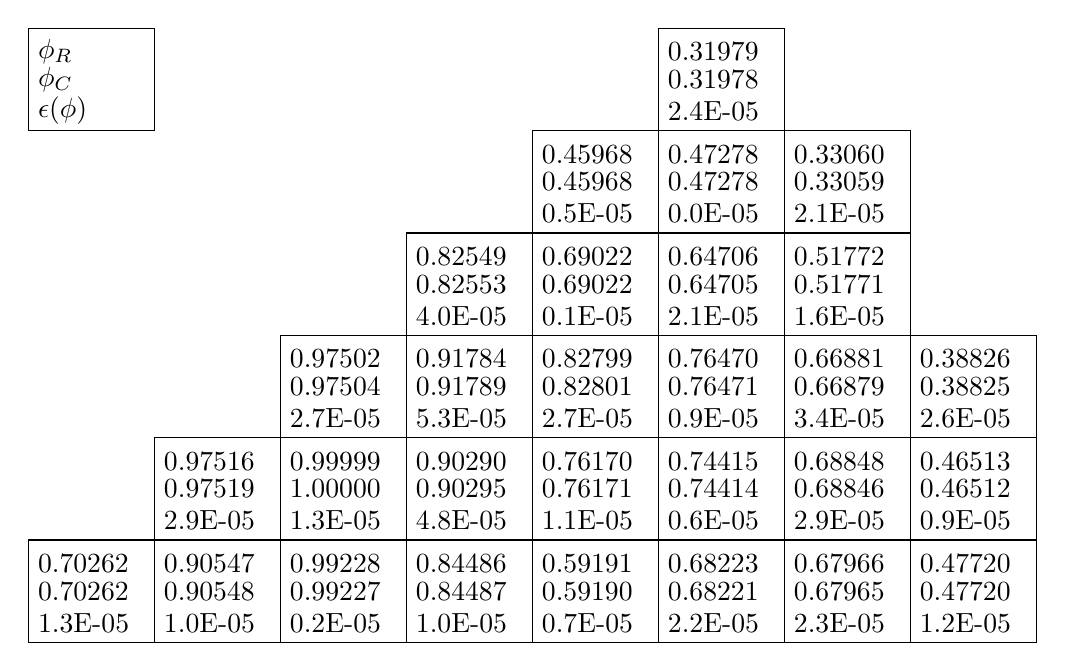
\begin{tikzpicture}
\def\di#1#2#3#4#5{
\def\boxx{1.6}
\def\boxy{1.3}
\draw (#1*\boxx, #2*\boxy) -- +(\boxx,0) -- +(\boxx,\boxy) -- +(0,\boxy) -- +(0,0);
\node [right] at (#1*\boxx,#2*\boxy+1) {#3};
\node [right]  at (#1*\boxx,#2*\boxy+0.65) {#4};
\node [right]  at (#1*\boxx,#2*\boxy+0.25) {#5};
}
\di{0}{5}{$\phi_R$}{$\phi_C$}{$\epsilon(\phi)$}
\di{0}{0}{0.70262}{0.70262}{1.3E-05}
\di{1}{0}{0.90547}{0.90548}{1.0E-05}
\di{1}{1}{0.97516}{0.97519}{2.9E-05}
\di{2}{0}{0.99228}{0.99227}{0.2E-05}
\di{2}{1}{0.99999}{1.00000}{1.3E-05}
\di{2}{2}{0.97502}{0.97504}{2.7E-05}
\di{3}{0}{0.84486}{0.84487}{1.0E-05}
\di{3}{1}{0.90290}{0.90295}{4.8E-05}
\di{3}{2}{0.91784}{0.91789}{5.3E-05}
\di{3}{3}{0.82549}{0.82553}{4.0E-05}
\di{4}{0}{0.59191}{0.59190}{0.7E-05}
\di{4}{1}{0.76170}{0.76171}{1.1E-05}
\di{4}{2}{0.82799}{0.82801}{2.7E-05}
\di{4}{3}{0.69022}{0.69022}{0.1E-05}
\di{4}{4}{0.45968}{0.45968}{0.5E-05}
\di{5}{0}{0.68223}{0.68221}{2.2E-05}
\di{5}{1}{0.74415}{0.74414}{0.6E-05}
\di{5}{2}{0.76470}{0.76471}{0.9E-05}
\di{5}{3}{0.64706}{0.64705}{2.1E-05}
\di{5}{4}{0.47278}{0.47278}{0.0E-05}
\di{5}{5}{0.31979}{0.31978}{2.4E-05}
\di{6}{0}{0.67966}{0.67965}{2.3E-05}
\di{6}{1}{0.68848}{0.68846}{2.9E-05}
\di{6}{2}{0.66881}{0.66879}{3.4E-05}
\di{6}{3}{0.51772}{0.51771}{1.6E-05}
\di{6}{4}{0.33060}{0.33059}{2.1E-05}
\di{7}{0}{0.47720}{0.47720}{1.2E-05}
\di{7}{1}{0.46513}{0.46512}{0.9E-05}
\di{7}{2}{0.38826}{0.38825}{2.6E-05}
\end{tikzpicture}
}

\subcaptionbox{热群}{
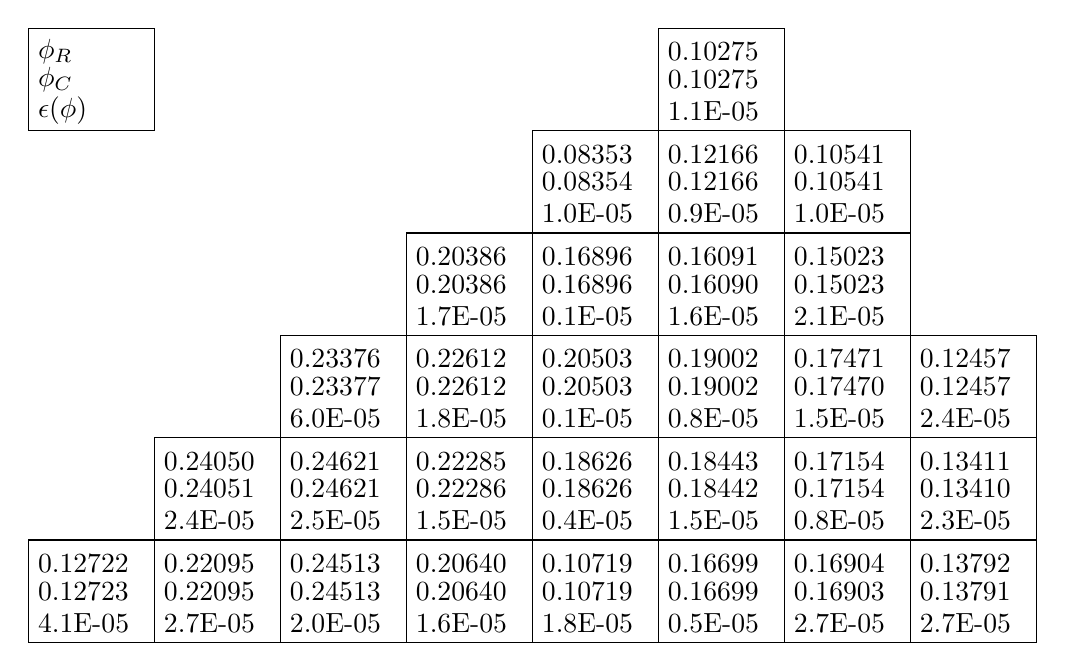
\begin{tikzpicture}
\def\di#1#2#3#4#5{
\def\boxx{1.6}
\def\boxy{1.3}
\draw (#1*\boxx, #2*\boxy) -- +(\boxx,0) -- +(\boxx,\boxy) -- +(0,\boxy) -- +(0,0);
\node [right] at (#1*\boxx,#2*\boxy+1) {#3};
\node [right]  at (#1*\boxx,#2*\boxy+0.65) {#4};
\node [right]  at (#1*\boxx,#2*\boxy+0.25) {#5};
}
\di{0}{5}{$\phi_R$}{$\phi_C$}{$\epsilon(\phi)$}
\di{0}{0}{0.12722}{0.12723}{4.1E-05}
\di{1}{0}{0.22095}{0.22095}{2.7E-05}
\di{1}{1}{0.24050}{0.24051}{2.4E-05}
\di{2}{0}{0.24513}{0.24513}{2.0E-05}
\di{2}{1}{0.24621}{0.24621}{2.5E-05}
\di{2}{2}{0.23376}{0.23377}{6.0E-05}
\di{3}{0}{0.20640}{0.20640}{1.6E-05}
\di{3}{1}{0.22285}{0.22286}{1.5E-05}
\di{3}{2}{0.22612}{0.22612}{1.8E-05}
\di{3}{3}{0.20386}{0.20386}{1.7E-05}
\di{4}{0}{0.10719}{0.10719}{1.8E-05}
\di{4}{1}{0.18626}{0.18626}{0.4E-05}
\di{4}{2}{0.20503}{0.20503}{0.1E-05}
\di{4}{3}{0.16896}{0.16896}{0.1E-05}
\di{4}{4}{0.08353}{0.08354}{1.0E-05}
\di{5}{0}{0.16699}{0.16699}{0.5E-05}
\di{5}{1}{0.18443}{0.18442}{1.5E-05}
\di{5}{2}{0.19002}{0.19002}{0.8E-05}
\di{5}{3}{0.16091}{0.16090}{1.6E-05}
\di{5}{4}{0.12166}{0.12166}{0.9E-05}
\di{5}{5}{0.10275}{0.10275}{1.1E-05}
\di{6}{0}{0.16904}{0.16903}{2.7E-05}
\di{6}{1}{0.17154}{0.17154}{0.8E-05}
\di{6}{2}{0.17471}{0.17470}{1.5E-05}
\di{6}{3}{0.15023}{0.15023}{2.1E-05}
\di{6}{4}{0.10541}{0.10541}{1.0E-05}
\di{7}{0}{0.13792}{0.13791}{2.7E-05}
\di{7}{1}{0.13411}{0.13410}{2.3E-05}
\di{7}{2}{0.12457}{0.12457}{2.4E-05}
\end{tikzpicture}
}
\caption{静态IAEA三维基准题\ProgramName 程序 CG-SG 1cm网格$1/8$堆芯组件通量相对偏差}
\label{fig:result.iaea.aphitable.cg}
\end{figure}


\begin{figure}
\centering
\subcaptionbox{快群}{
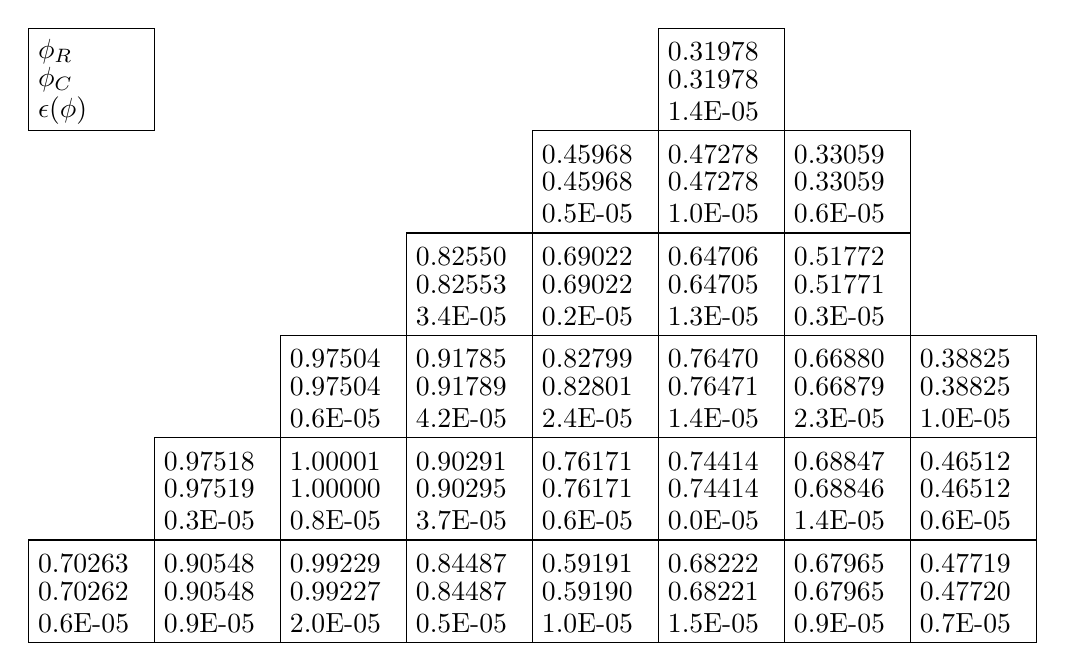
\begin{tikzpicture}
\def\di#1#2#3#4#5{
\def\boxx{1.6}
\def\boxy{1.3}
\draw (#1*\boxx, #2*\boxy) -- +(\boxx,0) -- +(\boxx,\boxy) -- +(0,\boxy) -- +(0,0);
\node [right] at (#1*\boxx,#2*\boxy+1) {#3};
\node [right]  at (#1*\boxx,#2*\boxy+0.65) {#4};
\node [right]  at (#1*\boxx,#2*\boxy+0.25) {#5};
}
\di{0}{5}{$\phi_R$}{$\phi_C$}{$\epsilon(\phi)$}
\di{0}{0}{0.70263}{0.70262}{0.6E-05}
\di{1}{0}{0.90548}{0.90548}{0.9E-05}
\di{1}{1}{0.97518}{0.97519}{0.3E-05}
\di{2}{0}{0.99229}{0.99227}{2.0E-05}
\di{2}{1}{1.00001}{1.00000}{0.8E-05}
\di{2}{2}{0.97504}{0.97504}{0.6E-05}
\di{3}{0}{0.84487}{0.84487}{0.5E-05}
\di{3}{1}{0.90291}{0.90295}{3.7E-05}
\di{3}{2}{0.91785}{0.91789}{4.2E-05}
\di{3}{3}{0.82550}{0.82553}{3.4E-05}
\di{4}{0}{0.59191}{0.59190}{1.0E-05}
\di{4}{1}{0.76171}{0.76171}{0.6E-05}
\di{4}{2}{0.82799}{0.82801}{2.4E-05}
\di{4}{3}{0.69022}{0.69022}{0.2E-05}
\di{4}{4}{0.45968}{0.45968}{0.5E-05}
\di{5}{0}{0.68222}{0.68221}{1.5E-05}
\di{5}{1}{0.74414}{0.74414}{0.0E-05}
\di{5}{2}{0.76470}{0.76471}{1.4E-05}
\di{5}{3}{0.64706}{0.64705}{1.3E-05}
\di{5}{4}{0.47278}{0.47278}{1.0E-05}
\di{5}{5}{0.31978}{0.31978}{1.4E-05}
\di{6}{0}{0.67965}{0.67965}{0.9E-05}
\di{6}{1}{0.68847}{0.68846}{1.4E-05}
\di{6}{2}{0.66880}{0.66879}{2.3E-05}
\di{6}{3}{0.51772}{0.51771}{0.3E-05}
\di{6}{4}{0.33059}{0.33059}{0.6E-05}
\di{7}{0}{0.47719}{0.47720}{0.7E-05}
\di{7}{1}{0.46512}{0.46512}{0.6E-05}
\di{7}{2}{0.38825}{0.38825}{1.0E-05}
\end{tikzpicture}
}

\subcaptionbox{热群}{
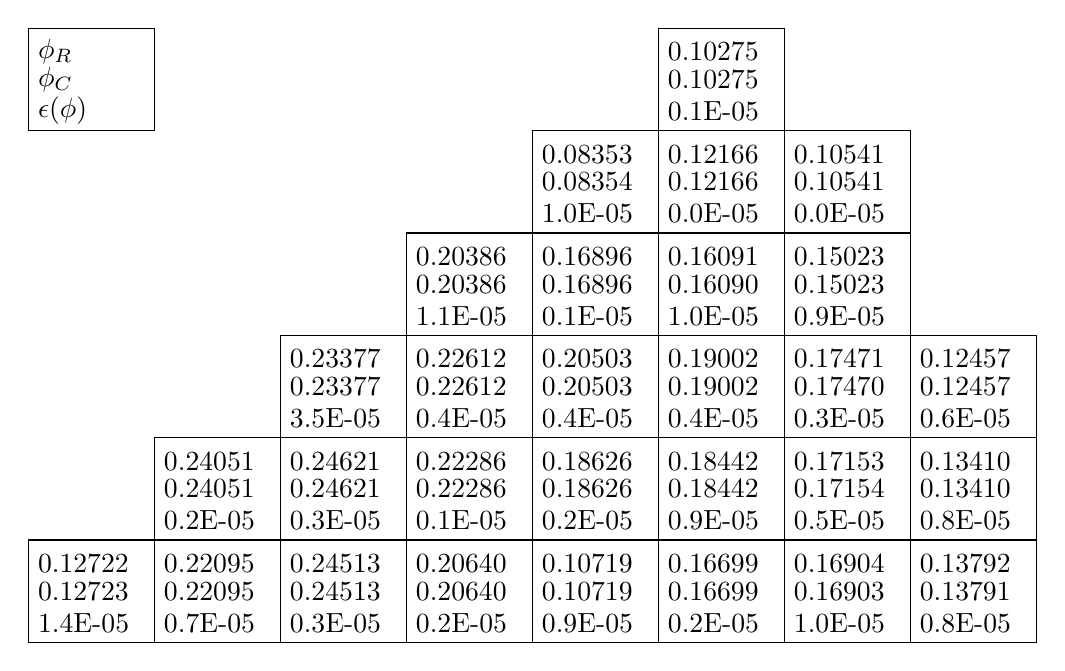
\begin{tikzpicture}
\def\di#1#2#3#4#5{
\def\boxx{1.6}
\def\boxy{1.3}
\draw (#1*\boxx, #2*\boxy) -- +(\boxx,0) -- +(\boxx,\boxy) -- +(0,\boxy) -- +(0,0);
\node [right] at (#1*\boxx,#2*\boxy+1) {#3};
\node [right]  at (#1*\boxx,#2*\boxy+0.65) {#4};
\node [right]  at (#1*\boxx,#2*\boxy+0.25) {#5};
}
\di{0}{5}{$\phi_R$}{$\phi_C$}{$\epsilon(\phi)$}
\di{0}{0}{0.12722}{0.12723}{1.4E-05}
\di{1}{0}{0.22095}{0.22095}{0.7E-05}
\di{1}{1}{0.24051}{0.24051}{0.2E-05}
\di{2}{0}{0.24513}{0.24513}{0.3E-05}
\di{2}{1}{0.24621}{0.24621}{0.3E-05}
\di{2}{2}{0.23377}{0.23377}{3.5E-05}
\di{3}{0}{0.20640}{0.20640}{0.2E-05}
\di{3}{1}{0.22286}{0.22286}{0.1E-05}
\di{3}{2}{0.22612}{0.22612}{0.4E-05}
\di{3}{3}{0.20386}{0.20386}{1.1E-05}
\di{4}{0}{0.10719}{0.10719}{0.9E-05}
\di{4}{1}{0.18626}{0.18626}{0.2E-05}
\di{4}{2}{0.20503}{0.20503}{0.4E-05}
\di{4}{3}{0.16896}{0.16896}{0.1E-05}
\di{4}{4}{0.08353}{0.08354}{1.0E-05}
\di{5}{0}{0.16699}{0.16699}{0.2E-05}
\di{5}{1}{0.18442}{0.18442}{0.9E-05}
\di{5}{2}{0.19002}{0.19002}{0.4E-05}
\di{5}{3}{0.16091}{0.16090}{1.0E-05}
\di{5}{4}{0.12166}{0.12166}{0.0E-05}
\di{5}{5}{0.10275}{0.10275}{0.1E-05}
\di{6}{0}{0.16904}{0.16903}{1.0E-05}
\di{6}{1}{0.17153}{0.17154}{0.5E-05}
\di{6}{2}{0.17471}{0.17470}{0.3E-05}
\di{6}{3}{0.15023}{0.15023}{0.9E-05}
\di{6}{4}{0.10541}{0.10541}{0.0E-05}
\di{7}{0}{0.13792}{0.13791}{0.8E-05}
\di{7}{1}{0.13410}{0.13410}{0.8E-05}
\di{7}{2}{0.12457}{0.12457}{0.6E-05}
\end{tikzpicture}
}
\caption{静态IAEA三维基准题\ProgramName 程序 CG-SG Multilevel 1cm网格$1/8$堆芯组件通量相对偏差}
\label{fig:result.iaea.aphitable.cgml}
\end{figure}

\subsection{动态TWIGL二维基准问题}

动态TWIGL二维基准题的计算结果及对比见\floatref{tab:result.twigl.power-compare},
可见\ProgramName 和各种节块程序的结果符合的较好。

\begin{table}
\centering
\begin{minipage}{\textwidth}
\centering
\caption{动态TWIGL二维基准问题计算结果(堆芯相对功率)\label{tab:result.twigl.power-compare}}
\subcaptionbox{阶跃反应性基准题\label{tab:result.twigl.power-compare.1}}
{
\begin{tabular}{cccccc}
\toprule
系统时刻/s & QUANDRY\footnote{使用解析节块法,时间步长0.01s,
             数据来源\onlinecite{smith1979analytic,zhaowenbo}。}
         & NEM\footnote{使用节块展开法,网格8cm$\times$8cm,时间步长0.005s,
             数据来源\onlinecite{bandini1990three,zhaowenbo}。}
         & NGFMN-K\footnote{使用节块格林函数法,网格8cm$\times$8cm,计算方法DIRK(5,4)-E,
             计算精度1e-5,数据来源\onlinecite{zhaowenbo}。}
         & SPANDEX\footnote{使用变时间步节块展开法,网格4cm$\times$4cm,时间步长0.0001s,
             数据来源\onlinecite{aviles1993development,sutton1996diffusion}。}
         & \ProgramName \footnote{本文工作,细网有限差分法,
             网格划分1cm$\times$1cm,时间步长$0.01$s。}
         \\
\midrule
0.1 & 2.064 & 2.060 & 2.061 & 2.062 & 2.060 \\
0.2 & 2.076 & 2.078 & 2.079 & 2.079 & 2.079 \\
0.3 & 2.095 & 2.095 & 2.096 & 2.096 & 2.096 \\
0.4 & 2.112 & 2.113 & 2.114 & 2.114 & 2.114 \\
0.5 & 2.130 & 2.131 & 2.131 & 2.131 & 2.131 \\
\bottomrule
\end{tabular}
}
\\[1cm]
\subcaptionbox{线性反应性基准题\label{tab:result.twigl.power-compare.2}}
{
\begin{tabular}{cccccc}
\toprule
系统时刻/s & QUANDRY\footnote{时间步长0.005s,
             数据来源\onlinecite{smith1979analytic,zhaowenbo}。}
         & NEM\footnote{网格8cm$\times$8cm,时间步长0.005s,
             数据来源\onlinecite{bandini1990three,zhaowenbo}。}
         & NGFMN-K\footnote{网格8cm$\times$8cm,计算方法DIRK(5,4)-E,
             计算精度1e-5,数据来源\onlinecite{zhaowenbo}。}
         & SPANDEX\footnote{网格4cm$\times$4cm,时间步长0.0001s,
             数据来源\onlinecite{aviles1993development,sutton1996diffusion}。}
         & \ProgramName \footnote{网格划分1cm$\times$1cm,时间步长$0.005$s。}
         \\
\midrule
0.1 & 1.305 & 1.309 & 1.309 & 1.309 & 1.309 \\
0.2 & 1.954 & 1.962 & 1.960 & 1.960 & 1.962 \\
0.3 & 2.074 & 2.075 & 2.075 & 2.075 & 2.076 \\
0.4 & 2.092 & 2.092 & 2.092 & 2.092 & 2.093 \\
0.5 & 2.109 & 2.110 & 2.110 & 2.110 & 2.111 \\
\bottomrule
\end{tabular}
}
\end{minipage}
\end{table}


\subsection{动态LMW三维基准问题}

动态LMW三维基准题的计算结果及对比见\floatref{tab:result.lmw.power-compare}。

\begin{sidewaystable}
\pdfrotate
\centering
\begin{minipage}{0.8\textwidth}
\centering
\caption{动态LMW三维基准问题计算结果(堆芯相对功率)}
\label{tab:result.lmw.power-compare}
\begin{tabular}{ccccccc}
\toprule
系统时刻/s & SKETCH-N\footnote{使用基于非线性迭代策略的CMFD方法,网格10cm$\times$10cm$\times$5cm,时间步长0.25s,
             数据来源\onlinecite{zimin1998nodal}。}
         & PANTHER\footnote{使用基于非线性迭代策略的解析节块法,网格10cm$\times$10cm$\times$5cm,时间步长0.25s,
             数据来源\onlinecite{sutton1996diffusion}。}
         & NGFMN-K\footnote{使用节块格林函数法,网格10cm$\times$10cm$\times$5cm,计算方法DIRK(5,4)-E,
             计算精度1e-5,数据来源\onlinecite{zhaowenbo}。}
         & SPANDEX\footnote{使用变时间步节块展开法,网格5cm$\times$5cm$\times$2.5cm,计算精度5e-2,
             数据来源\onlinecite{aviles1993development,sutton1996diffusion}。}
         & NLSANMT\footnote{使用基于非线性迭代策略的CMFD方法,网格10cm$\times$10cm$\times$5cm,时间步长0.25s,
             数据来源\onlinecite{liaochengkui,zhaowenbo}。}
         & \ProgramName \footnote{本文工作,细网有限差分法,
             网格划分1cm$\times$1cm$\times$1cm,时间步长$1/12$s。} 
         \\
\midrule
10 & 1.338 & 1.347 & 1.341 & 1.341 & 1.339 & 1.341\\
20 & 1.705 & 1.726 & 1.720 & 1.713 & 1.706 & 1.705\\
30 & 1.369 & 1.382 & 1.381 & 1.373 & 1.368 & 1.362\\
40 & 0.809 & 1.813 & 0.814 & 0.809 & 0.808 & 0.804\\
50 & 0.502 & 0.505 & 0.504 & 0.503 & 0.502 & 0.501\\
60 & 0.385 & 0.387 & 0.387 & 0.386 & 0.385 & 0.385\\ 
\bottomrule
\end{tabular}
\end{minipage}
\end{sidewaystable}


\FloatBarrier
\section{计算时间与加速效果分析}

\subsection{静态计算}

\begin{comment}

由于\ProgramName 和Citation均使用迭代算法进行求解,
而迭代算法的计算时间和通量的收敛程度有直接关系,
一般来说计算时间和迭代次数成正比。
但无论是计算本征值的外迭代还是求解线性方程的内迭代,
\ProgramName 和Citation都使用了不同的迭代方式,
两者对误差的估计方式也有所差别,不宜直接进行比较。

\begin{figure}
\centering
\includegraphics{testresult_iaea_1cm}
\caption{\label{fig:testresult.iaea}静态IAEA三维基准题1cm网格\ProgramName 与Citation的计算时间-通量最大偏差图}
\end{figure}

在实际应用中,相同误差时的计算时间才能反映程序间的速度差异,
这里分别选取不同的收敛精度使用\ProgramName 和Citation进行计算,
绘制两者的计算时间--偏差图,
这里取Citation在$\epsilon_\phi=5\times10^{-7}$时的计算结果作为参考值,
对于静态IAEA PWR 三维基准题1cm网格划分,
\ProgramName 与Citation在不同精度下的计算时间见\floatref{fig:testresult.iaea},
可见不同的算法的计算时间和结果精度的关系差异很大,对结果进行拟合得
\begin{align}
  &T_\mathrm{CG-SG\ ML} = \exp\pb{-0.235151\log \epsilon_\phi-146.097\epsilon_\phi+1.87266}\\
  &T_\mathrm{CG-SG} = \exp\pb{-0.307056\log \epsilon_\phi+2.02687} \\
  &T_\mathrm{Citation} = \exp\pb{-414.444\epsilon_\phi+10.7569} 
\end{align}
取结果偏差为$\epsilon_\phi=0.01,0.003,0.001$进行比较得

\begin{table}
\centering
\begin{tabular}{crrr}
\toprule
$\epsilon_\phi$ & $T_\mathrm{Citation}$ & $T_\mathrm{CG-SG\ ML}$ & $T_\mathrm{CG-SG}$\\
\midrule
0.01  &   744.31 &  4.46 & 31.22 \\
0.003 & 13542.20 & 16.45 & 45.18 \\
0.001 & 31022.10 & 28.53 & 63.30 \\
\bottomrule
\end{tabular}
\end{table}

\end{comment}

以静态IAEA PWR 三维基准题为例比较\ProgramName 和Citation程序的结果,
使用Citation程序在$\epsilon_\phi=5\times10^{-7}$时的计算结果作为参考值。
对于1cm网格,不同通量收敛精度下\ProgramName 和Citation程序的结果见\floatref{tab:testresult.iaea},
可见,相同的收敛精度下,CG-SG MultiLevel和CG-SG算法都明显快于Citation程序,
CG-SG MultiLevel的加速效果在52-272倍,CG-SG的加速效果在21-130倍,
$k_\mathrm{eff}$的收敛效果差于Citation程序,但也在$2\times10^{-5}$的范围内,
对于最大通量偏差,CG-SG MultiLevel和CG-SG算法的结果略好于Citation程序。

\begin{table}
\centering
\caption{\label{tab:testresult.iaea}静态IAEA三维基准题1cm网格\ProgramName 与Citation计算结果}
\begin{minipage}{\textwidth}
\centering
\begin{tabular}{cccccc}
\toprule
算法 & 通量收敛精度 & $T/s$ & $\epsilon_{k_\mathrm{eff}}$ & $\epsilon_{\phi_{\bm{k},g}}$ & 加速比\\
\midrule
Citation & $10^{-4}$ & 1338.96 & 8e-07\footnote{Citation只给出8位有效数字。} & 1.336767e-02 & --\\
Citation & $10^{-5}$ & 2143.08 & 5e-07 & 7.224095e-03 & --\\
Citation & $10^{-6}$ & 21437.00 & 0e-07 & 1.999625e-03 & --\\
CS-SG ML & $10^{-4}$ & 18.299 & 2.080200e-05 & 1.126408e-02 & 73.2\\
CS-SG ML & $10^{-5}$ & 41.215 & 1.003682e-05 & 1.322194e-03 & 52.0\\
CS-SG ML & $10^{-6}$ & 78.749 & 8.253441e-06 & 8.773718e-04 & 272.2\\
CS-SG & $10^{-4}$ &  48.376 & 1.939363e-05 & 2.183641e-02 & 27.7\\
CS-SG & $10^{-5}$ & 101.104 & 7.378584e-06 & 2.226546e-03 & 21.2\\
CS-SG & $10^{-6}$ & 164.877 & 8.031013e-06 & 1.035618e-03 & 130.0\\
\bottomrule
\end{tabular}
\end{minipage}
\end{table}


\subsection{时空动力学}

上一节中的时空动力学程序大多缺少和时间步对应的计算时间结果,
无法进行直接比较,这里只分析\ProgramName 程序自己的计算结果。

\subsubsection{动态TWIGL二维基准问题}

动态TWIGL二维基准题阶跃反应性计算结果见
\floatref{tab:testresult.twigl.1.1-2}和
\floatref{tab:testresult.twigl.1.4-8},
从结果中可以看出,网格大小放大为4cm时,
给定时刻的堆芯总功率偏差只有0.001左右,
网格大小进一步放大为8cm时,总功率偏差大约为0.02。
网格大小固定为4cm时,时间步长对总功率影响主要在第一个0.1s内,
步长从0.01放大到0.1的过程中,
0.1s时的堆芯总功率偏差逐渐达到0.09左右,
而0.2s时的堆芯总功率偏差最大只有0.09左右。
网格大小为4cm,时间步长取0.05s时,计算时间约等于模型时间,
基本达到实时模拟,此时最大总功率偏差出现在0.1s,偏差值约为0.03。

线性反应性计算结果见
\floatref{tab:testresult.twigl.2.1-2}和
\floatref{tab:testresult.twigl.2.4-8},
当网格大小放大到8cm时,总功率偏差值约有0.02。
固定网格大小为8cm后,调整时间步长,
总功率偏差主要出现在0.2s,偏差值最大达到0.04。
网格大小为2cm时间步长取0.10s时,
以及网格大小为4cm时间步长取0.05s时,能够实现实时模拟。


\begin{table}
\centering
\caption{动态TWIGL二维基准题阶跃反应性计算结果1\label{tab:testresult.twigl.1.1-2}}
\subcaptionbox{网格大小1cm 时间步长0.01s}
{
\small
\begin{tabular}{cccc}
\toprule
模型 & 堆芯 & 计算 & 累计计算\\
时间/s & 功率 & 时间/s & 时间/s\\
\midrule
init & 1.000 & -- & 1.825\\
0.1 & 2.060 & 1.700 & 3.525\\
0.2 & 2.079 & 1.482 & 5.007\\
0.3 & 2.096 & 1.513 & 6.520\\
0.4 & 2.114 & 1.544 & 8.064\\
0.5 & 2.131 & 1.496 & 9.560\\
\bottomrule
\end{tabular}
}
\subcaptionbox{网格大小1cm 时间步长0.02s}
{
\small
\begin{tabular}{cccc}
\toprule
模型 & 堆芯 & 计算 & 累计计算\\
时间/s & 功率 & 时间/s & 时间/s\\
\midrule
init & 1.000 & -- & 1.935\\
0.1 & 2.057 & 0.934 & 2.869\\
0.2 & 2.079 & 0.842 & 3.711\\
0.3 & 2.096 & 0.843 & 4.554\\
0.4 & 2.114 & 0.858 & 5.412\\
0.5 & 2.131 & 0.858 & 6.270\\
\bottomrule
\end{tabular}
}

\subcaptionbox{网格大小1cm 时间步长0.05s}
{
\small
\begin{tabular}{cccc}
\toprule
模型 & 堆芯 & 计算 & 累计计算\\
时间/s & 功率 & 时间/s & 时间/s\\
\midrule
init & 1.000 & -- & 1.887\\
0.1 & 2.031 & 0.390 & 2.277\\
0.2 & 2.078 & 0.359 & 2.636\\
0.3 & 2.096 & 0.343 & 2.979\\
0.4 & 2.114 & 0.343 & 3.322\\
0.5 & 2.131 & 0.358 & 3.680\\
\bottomrule
\end{tabular}
}
\subcaptionbox{网格大小1cm 时间步长0.10s}
{
\small
\begin{tabular}{cccc}
\toprule
模型 & 堆芯 & 计算 & 累计计算\\
时间/s & 功率 & 时间/s & 时间/s\\
\midrule
init & 1.000 & -- & 2.356\\
0.1 & 1.965 & 0.312 & 2.668\\
0.2 & 2.070 & 0.266 & 2.934\\
0.3 & 2.095 & 0.250 & 3.184\\
0.4 & 2.114 & 0.249 & 3.433\\
0.5 & 2.132 & 0.250 & 3.683\\
\bottomrule
\end{tabular}
}


\subcaptionbox{网格大小2cm 时间步长0.01s}
{
\small
\begin{tabular}{cccc}
\toprule
模型 & 堆芯 & 计算 & 累计计算\\
时间/s & 功率 & 时间/s & 时间/s\\
\midrule
init & 1.000 & -- & 1.497\\
0.1 & 2.060 & 0.811 & 2.308\\
0.2 & 2.078 & 0.700 & 3.008\\
0.3 & 2.096 & 0.684 & 3.692\\
0.4 & 2.113 & 0.732 & 4.424\\
0.5 & 2.131 & 0.764 & 5.188\\
\bottomrule
\end{tabular}
}
\subcaptionbox{网格大小2cm 时间步长0.02s}
{
\small
\begin{tabular}{cccc}
\toprule
模型 & 堆芯 & 计算 & 累计计算\\
时间/s & 功率 & 时间/s & 时间/s\\
\midrule
init & 1.000 & -- & 1.482\\
0.1 & 2.056 & 0.406 & 1.888\\
0.2 & 2.078 & 0.330 & 2.218\\
0.3 & 2.096 & 0.375 & 2.593\\
0.4 & 2.113 & 0.326 & 2.919\\
0.5 & 2.131 & 0.390 & 3.309\\
\bottomrule
\end{tabular}
}
\subcaptionbox{网格大小2cm 时间步长0.05s}
{
\small
\begin{tabular}{cccc}
\toprule
模型 & 堆芯 & 计算 & 累计计算\\
时间/s & 功率 & 时间/s & 时间/s\\
\midrule
init & 1.000 & -- & 1.482\\
0.1 & 2.031 & 0.172 & 1.654\\
0.2 & 2.077 & 0.156 & 1.810\\
0.3 & 2.096 & 0.124 & 1.934\\
0.4 & 2.113 & 0.156 & 2.090\\
0.5 & 2.131 & 0.156 & 2.246\\
\bottomrule
\end{tabular}
}
\subcaptionbox{网格大小2cm 时间步长0.10s}
{
\small
\begin{tabular}{cccc}
\toprule
模型 & 堆芯 & 计算 & 累计计算\\
时间/s & 功率 & 时间/s & 时间/s\\
\midrule
init & 1.000 & -- & 1.482\\
0.1 & 1.964 & 0.093 & 1.575\\
0.2 & 2.069 & 0.078 & 1.653\\
0.3 & 2.095 & 0.078 & 1.731\\
0.4 & 2.113 & 0.078 & 1.809\\
0.5 & 2.131 & 0.078 & 1.887\\
\bottomrule
\end{tabular}
}
\end{table}

\begin{table}
\centering
\caption{动态TWIGL二维基准题阶跃反应性计算结果2\label{tab:testresult.twigl.1.4-8}}
\subcaptionbox{网格大小4cm 时间步长0.01s}
{
\small
\begin{tabular}{cccc}
\toprule
模型 & 堆芯 & 计算 & 累计计算\\
时间/s & 功率 & 时间/s & 时间/s\\
\midrule
init & 1.000 & -- & 1.092\\
0.1 & 2.061 & 0.437 & 1.529\\
0.2 & 2.079 & 0.358 & 1.887\\
0.3 & 2.096 & 0.360 & 2.247\\
0.4 & 2.114 & 0.374 & 2.621\\
0.5 & 2.132 & 0.404 & 3.025\\
\bottomrule
\end{tabular}
}
\subcaptionbox{网格大小4cm 时间步长0.02s}
{
\small
\begin{tabular}{cccc}
\toprule
模型 & 堆芯 & 计算 & 累计计算\\
时间/s & 功率 & 时间/s & 时间/s\\
\midrule
init & 1.000 & -- & 1.169\\
0.1 & 2.057 & 0.265 & 1.434\\
0.2 & 2.079 & 0.249 & 1.683\\
0.3 & 2.096 & 0.219 & 1.902\\
0.4 & 2.114 & 0.234 & 2.136\\
0.5 & 2.132 & 0.250 & 2.386\\
\bottomrule
\end{tabular}
}

\subcaptionbox{网格大小4cm 时间步长0.05s}
{
\small
\begin{tabular}{cccc}
\toprule
模型 & 堆芯 & 计算 & 累计计算\\
时间/s & 功率 & 时间/s & 时间/s\\
\midrule
init & 1.000 & -- & 1.092\\
0.1 & 2.031 & 0.109 & 1.201\\
0.2 & 2.078 & 0.094 & 1.295\\
0.3 & 2.097 & 0.062 & 1.357\\
0.4 & 2.114 & 0.078 & 1.435\\
0.5 & 2.132 & 0.078 & 1.513\\
\bottomrule
\end{tabular}
}
\subcaptionbox{网格大小4cm 时间步长0.10s}
{
\small
\begin{tabular}{cccc}
\toprule
模型 & 堆芯 & 计算 & 累计计算\\
时间/s & 功率 & 时间/s & 时间/s\\
\midrule
init & 1.000 & -- & 1.232\\
0.1 & 1.965 & 0.062 & 1.294\\
0.2 & 2.070 & 0.047 & 1.341\\
0.3 & 2.096 & 0.047 & 1.388\\
0.4 & 2.114 & 0.031 & 1.419\\
0.5 & 2.132 & 0.031 & 1.450\\
\bottomrule
\end{tabular}
}


\subcaptionbox{网格大小8cm 时间步长0.01s}
{
\small
\begin{tabular}{cccc}
\toprule
模型 & 堆芯 & 计算 & 累计计算\\
时间/s & 功率 & 时间/s & 时间/s\\
\midrule
init & 1.000 & -- & 0.920\\
0.1 & 2.080 & 0.233 & 1.153\\
0.2 & 2.099 & 0.204 & 1.357\\
0.3 & 2.117 & 0.218 & 1.575\\
0.4 & 2.135 & 0.204 & 1.779\\
0.5 & 2.153 & 0.204 & 1.983\\
\bottomrule
\end{tabular}
}
\subcaptionbox{网格大小8cm 时间步长0.02s}
{
\small
\begin{tabular}{cccc}
\toprule
模型 & 堆芯 & 计算 & 累计计算\\
时间/s & 功率 & 时间/s & 时间/s\\
\midrule
init & 1.000 & -- & 0.889\\
0.1 & 2.076 & 0.126 & 1.015\\
0.2 & 2.099 & 0.110 & 1.125\\
0.3 & 2.117 & 0.110 & 1.235\\
0.4 & 2.135 & 0.095 & 1.330\\
0.5 & 2.153 & 0.095 & 1.425\\
\bottomrule
\end{tabular}
}
\subcaptionbox{网格大小8cm 时间步长0.05s}
{
\small
\begin{tabular}{cccc}
\toprule
模型 & 堆芯 & 计算 & 累计计算\\
时间/s & 功率 & 时间/s & 时间/s\\
\midrule
init & 1.000 & -- & 0.780\\
0.1 & 2.050 & 0.063 & 0.843\\
0.2 & 2.098 & 0.062 & 0.905\\
0.3 & 2.117 & 0.032 & 0.937\\
0.4 & 2.135 & 0.047 & 0.984\\
0.5 & 2.153 & 0.032 & 1.016\\
\bottomrule
\end{tabular}
}
\subcaptionbox{网格大小8cm 时间步长0.10s}
{
\small
\begin{tabular}{cccc}
\toprule
模型 & 堆芯 & 计算 & 累计计算\\
时间/s & 功率 & 时间/s & 时间/s\\
\midrule
init & 1.000 & -- & 0.795\\
0.1 & 1.982 & 0.031 & 0.826\\
0.2 & 2.089 & 0.031 & 0.857\\
0.3 & 2.116 & 0.016 & 0.873\\
0.4 & 2.135 & 0.015 & 0.888\\
0.5 & 2.153 & 0.015 & 0.903\\
\bottomrule
\end{tabular}
}
\end{table}

%-----------------------TWIGL 2-------------------------------------

\begin{table}
\centering
\caption{动态TWIGL二维基准题线性反应性计算结果1\label{tab:testresult.twigl.2.1-2}}
\subcaptionbox{网格大小1cm 时间步长0.005s}
{
\small
\begin{tabular}{cccc}
\toprule
模型 & 堆芯 & 计算 & 累计计算\\
时间/s & 功率 & 时间/s & 时间/s\\
\midrule
init & 1.000 & -- & 1.919\\
0.1 & 1.309 & 3.823 & 5.742\\
0.2 & 1.962 & 3.900 & 9.642\\
0.3 & 2.076 & 3.384 & 13.026\\
0.4 & 2.093 & 3.370 & 16.396\\
0.5 & 2.111 & 3.292 & 19.688\\
\bottomrule
\end{tabular}
}
\subcaptionbox{网格大小1cm 时间步长0.02s}
{
\small
\begin{tabular}{cccc}
\toprule
模型 & 堆芯 & 计算 & 累计计算\\
时间/s & 功率 & 时间/s & 时间/s\\
\midrule
init & 1.000 & -- & 2.137\\
0.1 & 1.311 & 0.982 & 3.119\\
0.2 & 1.969 & 1.279 & 4.398\\
0.3 & 2.077 & 0.890 & 5.288\\
0.4 & 2.095 & 0.795 & 6.083\\
0.5 & 2.112 & 0.843 & 6.926\\
\bottomrule
\end{tabular}
}

\subcaptionbox{网格大小1cm 时间步长0.05s}
{
\small
\begin{tabular}{cccc}
\toprule
模型 & 堆芯 & 计算 & 累计计算\\
时间/s & 功率 & 时间/s & 时间/s\\
\midrule
init & 1.000 & -- & 1.794\\
0.1 & 1.313 & 0.375 & 2.169\\
0.2 & 1.982 & 0.390 & 2.559\\
0.3 & 2.078 & 0.344 & 2.903\\
0.4 & 2.097 & 0.312 & 3.215\\
0.5 & 2.115 & 0.328 & 3.543\\
\bottomrule
\end{tabular}
}
\subcaptionbox{网格大小1cm 时间步长0.10s}
{
\small
\begin{tabular}{cccc}
\toprule
模型 & 堆芯 & 计算 & 累计计算\\
时间/s & 功率 & 时间/s & 时间/s\\
\midrule
init & 1.000 & -- & 1.825\\
0.1 & 1.318 & 0.218 & 2.043\\
0.2 & 2.000 & 0.203 & 2.246\\
0.3 & 2.079 & 0.172 & 2.418\\
0.4 & 2.102 & 0.156 & 2.574\\
0.5 & 2.120 & 0.156 & 2.730\\
\bottomrule
\end{tabular}
}


\subcaptionbox{网格大小2cm 时间步长0.005s}
{
\small
\begin{tabular}{cccc}
\toprule
模型 & 堆芯 & 计算 & 累计计算\\
时间/s & 功率 & 时间/s & 时间/s\\
\midrule
init & 1.000 & -- & 1.497\\
0.1 & 1.309 & 1.623 & 3.120\\
0.2 & 1.961 & 1.608 & 4.728\\
0.3 & 2.075 & 1.405 & 6.133\\
0.4 & 2.093 & 1.342 & 7.475\\
0.5 & 2.110 & 1.356 & 8.831\\
\bottomrule
\end{tabular}
}
\subcaptionbox{网格大小2cm 时间步长0.02s}
{
\small
\begin{tabular}{cccc}
\toprule
模型 & 堆芯 & 计算 & 累计计算\\
时间/s & 功率 & 时间/s & 时间/s\\
\midrule
init & 1.000 & -- & 1.513\\
0.1 & 1.310 & 0.421 & 1.934\\
0.2 & 1.968 & 0.437 & 2.371\\
0.3 & 2.076 & 0.390 & 2.761\\
0.4 & 2.094 & 0.390 & 3.151\\
0.5 & 2.112 & 0.342 & 3.493\\
\bottomrule
\end{tabular}
}
\subcaptionbox{网格大小2cm 时间步长0.05s}
{
\small
\begin{tabular}{cccc}
\toprule
模型 & 堆芯 & 计算 & 累计计算\\
时间/s & 功率 & 时间/s & 时间/s\\
\midrule
init & 1.000 & -- & 2.278\\
0.1 & 1.313 & 0.281 & 2.559\\
0.2 & 1.981 & 0.281 & 2.840\\
0.3 & 2.077 & 0.233 & 3.073\\
0.4 & 2.097 & 0.234 & 3.307\\
0.5 & 2.115 & 0.171 & 3.478\\
\bottomrule
\end{tabular}
}
\subcaptionbox{网格大小2cm 时间步长0.10s}
{
\small
\begin{tabular}{cccc}
\toprule
模型 & 堆芯 & 计算 & 累计计算\\
时间/s & 功率 & 时间/s & 时间/s\\
\midrule
init & 1.000 & -- & 1.576\\
0.1 & 1.318 & 0.094 & 1.670\\
0.2 & 1.999 & 0.093 & 1.763\\
0.3 & 2.078 & 0.094 & 1.857\\
0.4 & 2.102 & 0.078 & 1.935\\
0.5 & 2.120 & 0.078 & 2.013\\
\bottomrule
\end{tabular}
}
\end{table}

\begin{table}
\centering
\caption{动态TWIGL二维基准题线性反应性计算结果2\label{tab:testresult.twigl.2.4-8}}
\subcaptionbox{网格大小4cm 时间步长0.005s}
{
\small
\begin{tabular}{cccc}
\toprule
模型 & 堆芯 & 计算 & 累计计算\\
时间/s & 功率 & 时间/s & 时间/s\\
\midrule
init & 1.000 & -- & 1.217\\
0.1 & 1.309 & 0.998 & 2.215\\
0.2 & 1.962 & 1.122 & 3.337\\
0.3 & 2.076 & 0.857 & 4.194\\
0.4 & 2.094 & 0.716 & 4.910\\
0.5 & 2.111 & 0.826 & 5.736\\
\bottomrule
\end{tabular}
}
\subcaptionbox{网格大小4cm 时间步长0.02s}
{
\small
\begin{tabular}{cccc}
\toprule
模型 & 堆芯 & 计算 & 累计计算\\
时间/s & 功率 & 时间/s & 时间/s\\
\midrule
init & 1.000 & -- & 1.139\\
0.1 & 1.310 & 0.234 & 1.373\\
0.2 & 1.969 & 0.202 & 1.575\\
0.3 & 2.077 & 0.157 & 1.732\\
0.4 & 2.095 & 0.158 & 1.890\\
0.5 & 2.113 & 0.172 & 2.062\\
\bottomrule
\end{tabular}
}

\subcaptionbox{网格大小4cm 时间步长0.05s}
{
\small
\begin{tabular}{cccc}
\toprule
模型 & 堆芯 & 计算 & 累计计算\\
时间/s & 功率 & 时间/s & 时间/s\\
\midrule
init & 1.000 & -- & 1.107\\
0.1 & 1.313 & 0.094 & 1.201\\
0.2 & 1.982 & 0.094 & 1.295\\
0.3 & 2.078 & 0.063 & 1.358\\
0.4 & 2.098 & 0.078 & 1.436\\
0.5 & 2.115 & 0.063 & 1.499\\
\bottomrule
\end{tabular}
}
\subcaptionbox{网格大小4cm 时间步长0.10s}
{
\small
\begin{tabular}{cccc}
\toprule
模型 & 堆芯 & 计算 & 累计计算\\
时间/s & 功率 & 时间/s & 时间/s\\
\midrule
init & 1.000 & -- & 1.076\\
0.1 & 1.318 & 0.047 & 1.123\\
0.2 & 2.000 & 0.046 & 1.169\\
0.3 & 2.079 & 0.047 & 1.216\\
0.4 & 2.103 & 0.031 & 1.247\\
0.5 & 2.121 & 0.031 & 1.278\\
\bottomrule
\end{tabular}
}


\subcaptionbox{网格大小8cm 时间步长0.005s}
{
\small
\begin{tabular}{cccc}
\toprule
模型 & 堆芯 & 计算 & 累计计算\\
时间/s & 功率 & 时间/s & 时间/s\\
\midrule
init & 1.000 & -- & 0.780\\
0.1 & 1.312 & 0.359 & 1.139\\
0.2 & 1.978 & 0.390 & 1.529\\
0.3 & 2.096 & 0.374 & 1.903\\
0.4 & 2.114 & 0.359 & 2.262\\
0.5 & 2.132 & 0.328 & 2.590\\
\bottomrule
\end{tabular}
}
\subcaptionbox{网格大小8cm 时间步长0.02s}
{
\small
\begin{tabular}{cccc}
\toprule
模型 & 堆芯 & 计算 & 累计计算\\
时间/s & 功率 & 时间/s & 时间/s\\
\midrule
init & 1.000 & -- & 0.873\\
0.1 & 1.314 & 0.141 & 1.014\\
0.2 & 1.985 & 0.078 & 1.092\\
0.3 & 2.097 & 0.093 & 1.185\\
0.4 & 2.115 & 0.110 & 1.295\\
0.5 & 2.133 & 0.093 & 1.388\\
\bottomrule
\end{tabular}
}
\subcaptionbox{网格大小8cm 时间步长0.05s}
{
\small
\begin{tabular}{cccc}
\toprule
模型 & 堆芯 & 计算 & 累计计算\\
时间/s & 功率 & 时间/s & 时间/s\\
\midrule
init & 1.000 & -- & 0.857\\
0.1 & 1.316 & 0.063 & 0.920\\
0.2 & 1.998 & 0.062 & 0.982\\
0.3 & 2.098 & 0.047 & 1.029\\
0.4 & 2.118 & 0.047 & 1.076\\
0.5 & 2.136 & 0.032 & 1.108\\
\bottomrule
\end{tabular}
}
\subcaptionbox{网格大小8cm 时间步长0.10s}
{
\small
\begin{tabular}{cccc}
\toprule
模型 & 堆芯 & 计算 & 累计计算\\
时间/s & 功率 & 时间/s & 时间/s\\
\midrule
init & 1.000 & -- & 0.873\\
0.1 & 1.321 & 0.031 & 0.904\\
0.2 & 2.017 & 0.031 & 0.935\\
0.3 & 2.099 & 0.016 & 0.951\\
0.4 & 2.123 & 0.016 & 0.967\\
0.5 & 2.141 & 0.031 & 0.998\\
\bottomrule
\end{tabular}
}
\end{table}



\subsubsection{动态LMW三维基准问题}

动态LMW三维基准题计算结果见
\floatref{tab:testresult.lmw.size1}、
\floatref{tab:testresult.lmw.size2}、
\floatref{tab:testresult.lmw.size25}和
\floatref{tab:testresult.lmw.size5},
从结果可见,把空间网格放大到5cm时,
堆芯总功率的偏差值最大有0.03左右。
固定网格大小为5cm后,放大时间步长至1s,
总功率最大偏差放大到0.04左右,
时刻为30s。


\begin{table}
\centering
\caption{动态LMW三维基准题计算结果1\label{tab:testresult.lmw.size1}}
\subcaptionbox{网格大小1cm 时间步长1/12s}
{
\small
\begin{tabular}{cccc}
\toprule
模型 & 堆芯 & 计算 & 累计计算\\
时间/s & 功率 & 时间/s & 时间/s\\
\midrule
init & 1.000 & -- & 17.909\\
10.0 & 1.341 & 677.245 & 695.154\\
20.0 & 1.705 & 723.421 & 1418.575\\
30.0 & 1.362 & 714.762 & 2133.337\\
40.0 & 0.804 & 682.797 & 2816.134\\
50.0 & 0.501 & 658.147 & 3474.281\\
60.0 & 0.385 & 606.188 & 4080.469\\
\bottomrule
\end{tabular}
}
\subcaptionbox{网格大小1cm 时间步长1/6s}
{
\small
\begin{tabular}{cccc}
\toprule
模型 & 堆芯 & 计算 & 累计计算\\
时间/s & 功率 & 时间/s & 时间/s\\
\midrule
init & 1.000 & -- & 17.690\\
10.0 & 1.342 & 354.043 & 371.733\\
20.0 & 1.705 & 375.402 & 747.135\\
30.0 & 1.360 & 367.315 & 1114.450\\
40.0 & 0.803 & 353.246 & 1467.696\\
50.0 & 0.501 & 340.503 & 1808.199\\
60.0 & 0.385 & 306.380 & 2114.579\\
\bottomrule
\end{tabular}
}

\subcaptionbox{网格大小1cm 时间步长0.5s}
{
\small
\begin{tabular}{cccc}
\toprule
模型 & 堆芯 & 计算 & 累计计算\\
时间/s & 功率 & 时间/s & 时间/s\\
\midrule
init & 1.000 & -- & 17.815\\
10.0 & 1.349 & 131.836 & 149.651\\
20.0 & 1.711 & 133.583 & 283.234\\
30.0 & 1.356 & 133.971 & 417.205\\
40.0 & 0.799 & 132.957 & 550.162\\
50.0 & 0.500 & 124.378 & 674.540\\
60.0 & 0.384 & 104.364 & 778.904\\
\bottomrule
\end{tabular}
}
\subcaptionbox{网格大小1cm 时间步长1s}
{
\begin{tabular}{cccc}
\toprule
模型 & 堆芯 & 计算 & 累计计算\\
时间/s & 功率 & 时间/s & 时间/s\\
\midrule
init & 1.000 & -- & 18.080\\
10.0 & 1.353 & 67.923 & 86.003\\
20.0 & 1.710 & 69.591 & 155.594\\
30.0 & 1.344 & 68.671 & 224.265\\
40.0 & 0.790 & 67.079 & 291.344\\
50.0 & 0.496 & 65.100 & 356.444\\
60.0 & 0.382 & 56.755 & 413.199\\
\bottomrule
\end{tabular}
}
\end{table}

\begin{table}
\centering
\caption{动态LMW三维基准题计算结果2\label{tab:testresult.lmw.size2}}
\subcaptionbox{网格大小2cm 时间步长1/12s}
{
\small
\begin{tabular}{cccc}
\toprule
模型 & 堆芯 & 计算 & 累计计算\\
时间/s & 功率 & 时间/s & 时间/s\\
\midrule
init & 1.000 & -- & 7.816\\
10.0 & 1.341 & 64.663 & 72.479\\
20.0 & 1.703 & 69.853 & 142.332\\
30.0 & 1.360 & 67.894 & 210.226\\
40.0 & 0.803 & 67.125 & 277.351\\
50.0 & 0.501 & 65.412 & 342.763\\
60.0 & 0.385 & 62.287 & 405.050\\
\bottomrule
\end{tabular}
}
\subcaptionbox{网格大小2cm 时间步长1/6s}
{
\small
\begin{tabular}{cccc}
\toprule
模型 & 堆芯 & 计算 & 累计计算\\
时间/s & 功率 & 时间/s & 时间/s\\
\midrule
init & 1.000 & -- & 7.815\\
10.0 & 1.342 & 33.745 & 41.560\\
20.0 & 1.706 & 36.989 & 78.549\\
30.0 & 1.360 & 35.520 & 114.069\\
40.0 & 0.802 & 35.101 & 149.170\\
50.0 & 0.500 & 34.196 & 183.366\\
60.0 & 0.384 & 31.747 & 215.113\\
\bottomrule
\end{tabular}
}

\subcaptionbox{网格大小2cm 时间步长0.5s}
{
\small
\begin{tabular}{cccc}
\toprule
模型 & 堆芯 & 计算 & 累计计算\\
时间/s & 功率 & 时间/s & 时间/s\\
\midrule
init & 1.000 & -- & 7.612\\
10.0 & 1.348 & 12.260 & 19.872\\
20.0 & 1.711 & 12.825 & 32.697\\
30.0 & 1.356 & 12.371 & 45.068\\
40.0 & 0.799 & 12.246 & 57.314\\
50.0 & 0.499 & 11.637 & 68.951\\
60.0 & 0.384 & 10.325 & 79.276\\
\bottomrule
\end{tabular}
}
\subcaptionbox{网格大小2cm 时间步长1s}
{
\begin{tabular}{cccc}
\toprule
模型 & 堆芯 & 计算 & 累计计算\\
时间/s & 功率 & 时间/s & 时间/s\\
\midrule
init & 1.000 & -- & 7.722\\
10.0 & 1.359 & 6.614 & 14.336\\
20.0 & 1.725 & 6.598 & 20.934\\
30.0 & 1.361 & 6.457 & 27.391\\
40.0 & 0.802 & 6.351 & 33.742\\
50.0 & 0.503 & 6.159 & 39.901\\
60.0 & 0.387 & 5.520 & 45.421\\
\bottomrule
\end{tabular}
}
\end{table}

\begin{table}
\centering
\caption{动态LMW三维基准题计算结果3\label{tab:testresult.lmw.size25}}
\subcaptionbox{网格大小2.5cm 时间步长1/12s}
{
\small
\begin{tabular}{cccc}
\toprule
模型 & 堆芯 & 计算 & 累计计算\\
时间/s & 功率 & 时间/s & 时间/s\\
\midrule
init & 1.000 & -- & 3.978\\
10.0 & 1.341 & 34.352 & 38.330\\
20.0 & 1.707 & 36.424 & 74.754\\
30.0 & 1.365 & 35.536 & 110.290\\
40.0 & 0.805 & 35.666 & 145.956\\
50.0 & 0.501 & 34.881 & 180.837\\
60.0 & 0.384 & 33.381 & 214.218\\
\bottomrule
\end{tabular}
}
\subcaptionbox{网格大小2.5cm 时间步长1/6s}
{
\small
\begin{tabular}{cccc}
\toprule
模型 & 堆芯 & 计算 & 累计计算\\
时间/s & 功率 & 时间/s & 时间/s\\
\midrule
init & 1.000 & -- & 4.165\\
10.0 & 1.342 & 19.022 & 23.187\\
20.0 & 1.708 & 20.409 & 43.596\\
30.0 & 1.364 & 20.045 & 63.641\\
40.0 & 0.805 & 19.791 & 83.432\\
50.0 & 0.501 & 19.469 & 102.901\\
60.0 & 0.384 & 18.248 & 121.149\\
\bottomrule
\end{tabular}
}

\subcaptionbox{网格大小2.5cm 时间步长0.5s}
{
\small
\begin{tabular}{cccc}
\toprule
模型 & 堆芯 & 计算 & 累计计算\\
时间/s & 功率 & 时间/s & 时间/s\\
\midrule
init & 1.000 & -- & 3.932\\
10.0 & 1.346 & 6.707 & 10.639\\
20.0 & 1.714 & 6.865 & 17.504\\
30.0 & 1.364 & 6.895 & 24.399\\
40.0 & 0.804 & 6.862 & 31.261\\
50.0 & 0.501 & 6.599 & 37.860\\
60.0 & 0.385 & 5.928 & 43.788\\
\bottomrule
\end{tabular}
}
\subcaptionbox{网格大小2.5cm 时间步长1s}
{
\begin{tabular}{cccc}
\toprule
模型 & 堆芯 & 计算 & 累计计算\\
时间/s & 功率 & 时间/s & 时间/s\\
\midrule
init & 1.000 & -- & 3.900\\
10.0 & 1.353 & 3.573 & 7.473\\
20.0 & 1.718 & 3.665 & 11.138\\
30.0 & 1.358 & 3.683 & 14.821\\
40.0 & 0.800 & 3.540 & 18.361\\
50.0 & 0.500 & 3.542 & 21.903\\
60.0 & 0.385 & 3.056 & 24.959\\
\bottomrule
\end{tabular}
}
\end{table}

\begin{table}
\centering
\caption{动态LMW三维基准题计算结果4\label{tab:testresult.lmw.size5}}
\subcaptionbox{网格大小5cm 时间步长1/12s}
{
\small
\begin{tabular}{cccc}
\toprule
模型 & 堆芯 & 计算 & 累计计算\\
时间/s & 功率 & 时间/s & 时间/s\\
\midrule
init & 1.000 & -- & 2.933\\
10.0 & 1.337 & 9.435 & 12.368\\
20.0 & 1.686 & 10.111 & 22.479\\
30.0 & 1.342 & 9.909 & 32.388\\
40.0 & 0.795 & 10.015 & 42.403\\
50.0 & 0.501 & 9.625 & 52.028\\
60.0 & 0.385 & 8.782 & 60.810\\
\bottomrule
\end{tabular}
}
\subcaptionbox{网格大小5cm 时间步长1/6s}
{
\small
\begin{tabular}{cccc}
\toprule
模型 & 堆芯 & 计算 & 累计计算\\
时间/s & 功率 & 时间/s & 时间/s\\
\midrule
init & 1.000 & -- & 2.979\\
10.0 & 1.339 & 4.708 & 7.687\\
20.0 & 1.685 & 5.179 & 12.866\\
30.0 & 1.339 & 5.051 & 17.917\\
40.0 & 0.793 & 4.963 & 22.880\\
50.0 & 0.501 & 4.899 & 27.779\\
60.0 & 0.385 & 4.492 & 32.271\\
\bottomrule
\end{tabular}
}

\subcaptionbox{网格大小5cm 时间步长0.5s}
{
\small
\begin{tabular}{cccc}
\toprule
模型 & 堆芯 & 计算 & 累计计算\\
时间/s & 功率 & 时间/s & 时间/s\\
\midrule
init & 1.000 & -- & 2.949\\
10.0 & 1.344 & 1.733 & 4.682\\
20.0 & 1.686 & 1.887 & 6.569\\
30.0 & 1.331 & 1.811 & 8.380\\
40.0 & 0.789 & 1.779 & 10.159\\
50.0 & 0.500 & 1.652 & 11.811\\
60.0 & 0.385 & 1.638 & 13.449\\
\bottomrule
\end{tabular}
}
\subcaptionbox{网格大小5cm 时间步长1s}
{
\begin{tabular}{cccc}
\toprule
模型 & 堆芯 & 计算 & 累计计算\\
时间/s & 功率 & 时间/s & 时间/s\\
\midrule
init & 1.000 & -- & 2.965\\
10.0 & 1.346 & 0.920 & 3.885\\
20.0 & 1.683 & 0.996 & 4.881\\
30.0 & 1.318 & 0.983 & 5.864\\
40.0 & 0.780 & 0.983 & 6.847\\
50.0 & 0.496 & 0.921 & 7.768\\
60.0 & 0.382 & 0.874 & 8.642\\
\bottomrule
\end{tabular}
}
\end{table}
